% * LATEX definitions
\documentclass[aps,preprint,superscriptaddress]{revtex4-1}

\usepackage[english]{babel}
%\usepackage[latin1]{inputenc}
\usepackage{graphicx}
\usepackage{amsmath}
%\usepackage{fixmath}
\usepackage{color}
\usepackage{bm}
\usepackage{xcolor}
\usepackage{hyperref}
\usepackage{todonotes}
\hypersetup{
    colorlinks,
    linkcolor={red!50!black},
    citecolor={blue!50!black},
    urlcolor={blue!80!black}
}

% * my own definitions below.
\def\inst{}
\def\typeofdoc{}
\def\course{}
%\def\title{}
\def\name{}
%\def\email{}
\def\graders{\textbf{}}
\def\supervisors{\textbf{}}
\def\Li{\mathrm{Li}}
\def\d{\mathrm{d}}
\def\xx{\mathbf{x}}
\def\jj{\mathbf{j}}
\def\EE{\mathbf{E}}
\def\vv{\mathbf{v}}
\def\PP{\mathbf{P}}
\def\pp{\mathbf{p}}
\def\qq{\mathbf{q}}
\def\ll{\mathbf{l}}
\def\kk{\mathbf{k}}
\def\GG{\mathbf{G}}
\def\bb{\mathbf{b}}
\def\rr{\mathbf{r}}
\def\Rarrow{\Rightarrow}
\newcommand{\mrm}[1]{\mathrm{#1}}
\newcommand{\mbf}[1]{\mathbf{#1}}
\def\xhat{\mbf{\hat{x}}}
\def\yhat{\mbf{\hat{y}}}
\def\zhat{\mbf{\hat{z}}}
\def\Ordo{\mathcal{O}}
\def\Lag{\mathcal{L}}
\def\beq{\begin{equation}}
\def\eeq{\end{equation}}
\newcommand{\pd}[2]{\frac{\partial #1}{\partial #2}}
\newcommand{\fd}[2]{\frac{\delta #1}{\delta #2}}
\def\bdm{\begin{displaymath}}
\def\edm{\end{displaymath}}
\def\Mtot{M_{\mathrm{tot}}}
\newcommand{\nb}[1]{\textcolor{magenta}{\emph{[#1]}}}
\newcommand{\Qc}[0]{Q_\mrm{c}}
\newcommand{\Qp}[0]{Q_\mrm{p}}
\newcommand{\Sp}[0]{S_\mrm{p}}
\newcommand{\Sc}[0]{S_\mrm{c}}
\newcommand{\mR}[0]{m_\mrm{R}}
\newcommand{\kC}[0]{k_\mrm{C}}
\newcommand{\Zp}[0]{Z_\mrm{p}}
\newcommand{\Zc}[0]{Z_\mrm{c}}
\newcommand{\Stot}[0]{S_\mrm{tot}}
\def\bea{\begin{eqnarray}}
\def\eea{\end{eqnarray}}
\newcommand{\newrow}[1]{\nonumber\\&&#1}

\begin{document}

% * Title Page
\title{The short-range effective field theory with van der Waals tail
  at next-to-leading order} \author{Daniel Odell}
\email{dodell@ohio.edu} \affiliation{Department of Physics and
  Astronomy, University of Tennessee, Knoxville, TN 37996, USA}
\affiliation{Department of Physics and Astronomy, Ohio University,
  Athens, OH 45701, USA} \author{Arnoldas Deltuva}
\affiliation{Institute of Theoretical Physics and Astronomy, Vilnius
  University, Saul\.etekio al. 3, LT-10257 Vilnius, Lithuania}
\author{Lucas Platter} \email{lplatter@utk.edu}
\affiliation{Department of Physics and Astronomy, University of
  Tennessee, Knoxville, TN 37996, USA} \affiliation{Physics Division,
  Oak Ridge National Laboratory, Oak Ridge, TN 37831, USA}
\date{\today}

\listoftodos

\begin{abstract}
  We construct the first subleading correction in an effective field
  theory with short-range interactions and a van der Waals tail. We
  analyze the of the coupling constants with the short-distance
  regulator necessary within this framework. We study the size of the
  corrections that such a next-to-leading order term gives and argue
  that a counting for higher order corrections should be done on the
  basis of a modified effective range expansion. Furthermore, we
  discuss constraints on the next-to-leading oder correction imposed
  by causality and consider some physically relevant two-body
  examples. Finally, we use this interaction to analyze subleading
  corrections in the three-body sector.
\end{abstract}

\smallskip
\maketitle
%\tableofcontents

\newpage
%%%%%%%%%%%%%%%%%%%%%% 
% * Introduction
%%%%%%%%%%%%%%%%%%%%%
\section{Introduction}
\label{sec:introduction}
The long-range part of the interaction between atoms is frequently the
van der Waals interaction (vdW), {\it i.e.} $1/r^6$, where $r$ denotes
the relative distance between two atoms. Frequently, this vdW part is
combined with a more complicated short-distance form to construct
models [[REF he4]] intended to describe observables of these systems
to high accuracy.

An alternative approach to construct an Hamiltonian for atoms
interacting at long distances through a vdW tail is to build an
effective interaction. Such an interaction whose construction uses
simple building blocks and is based on simple principles promises a 

This approach is very similar in spirit to the quantum defect theory
that has been applied to the vdW problem by Bo Gao to derive the
two-body wave functions of two particles interacting through a vdW
potential~\cite{PhysRevA.58.1728}.

Recently, we evaluated the potential of such an effective theory
approach using the $^4$He dimer and trimer system as our benchmark
system \cite{Odell:2021ryo}. We found that a regularized and
renormalized interaction vdW interaction with one short-distance
counterterm can describe these systems very well.[[expand]]k

In this manuscript, we will extend the work started in
Ref.~\cite{Odell:2021ryo} and include the first subleading correction
in $S$- and $P$-waves. We will focus on systems with a large
scattering length in the S-wave and a large scattering volume in the
P-wave and discuss the implications of Gao's work for these system. We
will also address the constraints imposed by causality onto such an
approach.  Furthermore, we will construct the interaction that can be
used in a momentum space formalism to calculate observables of two-
but also higher-body systems. Since the vdW is singular, we will also
explain how this interaction is regularized and renormalized. We will
then again display how causality expresses itself in renormalized observables.

%%%%%%%%%%%%%%%%%%%%%%%%
% * Potential 
\section{Quantum defect theory for the van der Waals interaction}
\label{sec:vdw-interaction}
%%%%%%%%%%%%%%%%%%%%%%%%%%%%%
% ** Previous work
\subsection{The van der Waals two-body wave functions}
\label{sec:gao}
In Refs.~\cite{PhysRevA.58.1728}, Gao derived exact solution for the
two-body system interacting through a van der Waals interaction of the
form
\begin{equation}
  \label{eq:v_vdW}
  V(r) = -\frac{C_6}{r^6}~.
\end{equation}

Change this section to include an NLO discussion:
\begin{itemize}
\item  What happens if we include K2 in the Gao stuff.
\item What does Konigs work imply for K2 and thereby for the effective
  range. We can derive formulas that givegx explicit bounds close to the
  resonance. This would be a new result.
\item What happens close to resonance. Discuss that linear terms in
  P-wave drops out. I think non-analytic pieces also drop out in the
  S-wave. Is this a general feature? What happens for example in the
  D-wave? 
\end{itemize}


The van der Waals {\it strength} $C_6$ can be converted into a {\it
  characteristic} length scale $\beta_6\equiv {(mC_6)}^{1/4}$, where
$m$ is the mass of the interacting particles. Gao derived solutions
to the attractive $1/r^6$ potential in
Ref.~\cite{PhysRevA.58.1728}. The bound state wave function of the
state with energy $E$ in partial wave $l$ is written as the linear
combination of two solutions,$f_{E l}(r) $ and $g_{E l}(r$ of the
van der Waals interaction
\begin{equation}
  \label{eq:GaoSol}
  u_{E l}(r) = A_{E l}\left[f_{E l}(r) - K_l g_{E l}(r)\right]~,
\end{equation}
where $A_{E l}$ is a normalization coefficient and $K_l$ denotes the
so-called short-range K-matrix that fixes here an additional boundary
condition on the wave function that is required due to the
potentials's singularity at its origin. The precise forms of the
functions $f_{E l}(r)$ and $g_{E l}(r)$ are given in
Ref.~\cite{PhysRevA.58.1728}. For bound states, their asymptotic
form is given by
\begin{align}
  \label{eq:GaoAsym}
  f_{El}(r) \rightarrow {(2\pi \kappa)}^{-1/2} (W_{f-}e^{\kappa r} +
  W_{f+}e^{-\kappa r})~, \nonumber \\
  g_{El}(r) \rightarrow {(2\pi \kappa)}^{-1/2} (W_{g-}e^{\kappa r} +
  W_{g+}e^{\kappa r})~,
\end{align}
where $\kappa$ represents the bound state momentum and the
coefficients $W_{f\pm,g\pm}$ depend on the energy, $E$,
and the angular momentum, $l$, of the of bound state \cite{PhysRevA.58.1728}.

Requiring Eq.~\eqref{eq:GaoSol} to give normalizable solution implies
that the terms proportional to $e^{\kappa r}$ in
Eq.~\eqref{eq:GaoAsym} cancel and leads to
\begin{equation}
  \label{eq:chi}
  K_l(E) = \chi_l(\Delta) = W_{f-}/W_{g-}~,
\end{equation}
where $\Delta = 2\mu E \beta_6^2/16\hbar^2$.

The solid line in Fig.~\ref{fig:chi} shows the function
$\chi_{l=0}(\Delta)$ for an arbitrary value $\beta_6$. The
intersections between the dashed line and the solid line give the
two-body binding energies in terms of the rescaled energy variable
$\Delta$ once the boundary condition is chosen either by adjusting the
energy ($\Delta$) - position of one the intersections or by adjusting
a scattering observable.

Expressions for the asymptotic solutions at positive energies can be
used to derive expressions for the two-body t-matrix and thereby for
the effective range parameters. Gao obtains for the S-wave scattering
length and effective range~\cite{PhysRevA.58.4222}
\begin{equation}
  \begin{split}
    \label{eq:gao_a_and_r}
      a_s & = \frac{2\pi}{{[\Gamma(1/4)]}^2}\frac{K_0(0) -
        1}{K_0(0)}\, \beta_6~, \\
      r_s & \approx \frac{{[\Gamma(1/4)]}^2}{3\pi} \frac{K_0{(0)}^2 +
        1}{{[K_0(0)-1]}^2}\, \beta_6~,
  \end{split}
\end{equation}
where the $K_l(0)$ is evaluated at zero energy (threshold).  The
relation for $r_0$ is truncated under the assumption that the
derivative of the short-range $K$-matrix is small.  In effect, we can
calculate the boundary condition, $K_0(0)$, from $a$, and then
calculate $r_0$.

The scattering length is then dependent on the van der Waals length scale,
$\beta_6$ and the short-range $K$-matrix, $K_{l}$, evaluated in the $s$-wave
channel at zero energy.
\section{Renormalization of singular potentials}
We discussed above that Gao derived a solution for the van der Waals
interaction and that the parameters that map these solutions on a
physical system, are in Gao's work through an analytic function $K(E)$
that can be expanded when the energy dependence is {\it slow}.

Here, we want to figure out 


\begin{itemize}
\item We will assume that scattering length is large compared to the van der
  Waals length scale. This fixes the boundary condition at 0 energy
  and determines the existence of a shallow bound state.
\item We also assume that the potential is a pure $1/r^6$ from
  $\infty$ until much smaller distances.
\item Only causality limits the effective range through the Wigner
  bound.
\item Boundary condition is a function of the energy K(E) can in
  principle have arbitrary form. This also means that it can vary
  strongly. According to Gao, the function K is analytic in the
  energy. That means for every possible function $K$, there is an
  expansion in the energy with some convergence radius.
\item In Gao’s language, the intercepts of the function $\chi(E)$ and
  K(E) determine the bound state spectrum
\end{itemize}

We find that
\begin{itemize}
\item Iterating the interaction and running the (energy-independent)
  regulator $\Lambda$, corresponds to running through a class of
  short-range interactions (vs. the long-range tail) with a single
  parameter. This can lead to additional fine tunings that imply that
  mapping this interaction will have a large expansion parameter
  $K_n$.
\end{itemize}

\subsection{Renormalization with one counterterm (leading order)}


\subsection{Renormalization with two counterterms (next-to-leading
  order)}
\begin{figure}[t]
\begin{center}
\includegraphics[width=0.6\textwidth,clip=true]{image} 
\end{center}
\caption{Bound state spectrum as a function of the regulator $R$.}
\label{fig:bs-spectrum-lo}
\end{figure}
Figure~\ref{fig:bs-spectrum-lo} shows the bound state spectrum from a
calculation with 2 counterterms on a linear scale. The blue circles
give the results of the calculation with one counterterm (LO) tuned to
give the LM2M2 scatering length. The orange crosses give the bound
state spectrum obtained with two counterterms tuned to give the LM2M2
scattering length and effective range.

\begin{figure}[t]
\begin{center}
\includegraphics[width=0.6\textwidth,clip=true]{image-nlo} 
\end{center}
\caption{Spectrum}
\label{fig:bs-spectrum-nlo}
\end{figure}

Figure~\ref{fig:bs-spectrum-nlo}

% * The Wigner bound at unitarity
\section{The Wigner Bound at Unitarity}
\label{sec:wigner-bound-at-unitarity}
Elhatisari {\it et al.}~\cite{Elhatisari:2013swa} took the expansion
of the short-range $K$ matrix
\begin{equation}
  \label{eq:K_expansion}
  K^{(0)} = \tan\delta_{\ell}^{({\rm short})}(k) = \sum_{n=0}^\infty
  K_{\ell,2n}k^{2n}~,
\end{equation}
and derived a causality bound on the second coefficient of the expansion, given
by
\begin{equation}
  K_{\ell,2} \le b_{\ell}(r)~.
\end{equation}
This constraint on the subleading coefficient of the short-range
K-matrix limits the values of the effective range. Below we will
discuss the implications for S- and P-waves.

\subsection{$S$ Waves}
Gao derived the scattering phaseshifts using the exact solutions of
the wave functions of the two-body system interacting through a van
der Waals interaction
\begin{multline}
  \label{eq:kcotd-Swave}
(\beta_6 k) \cot\delta = \left[-\frac{(\beta_6 k)^2}{3}-\frac{1}{90} \pi  \beta_6 ^6 k^6 \left(K-\frac{181}{70 \pi }\right)-\frac{11}{900} \beta_6 ^4 k^4 \left(K-\frac{30 \pi
   }{11}\right)+\frac{2 \pi ^2 \beta_6 ^5 k^5 (K-1)}{15 \Gamma
   \left(\frac{1}{4}\right)^2}-K\right]\\
\times \Biggl\{
 \frac{1}{\Gamma \left(\frac{1}{4}\right)^2}\Biggl[2 \pi  \left(-\frac{4}{15} \beta_6 ^4 k^4 \log (\beta_6 
   k)+\frac{2}{15} \beta_6 ^4 k^4 \left(\frac{22}{5}-\gamma +\log
     (2)\right)+1\right)
 \\
 \times\biggl(-\frac{1}{90} \pi  \beta_6 ^6 k^6 \bigl(K+\frac{181 (K+1)}{70 \pi
     }-1\bigr)\\
   +\frac{11}{900} \beta_6 ^4 k^4 \bigl(K+\frac{30}{11} \pi
   (K+1)-1\bigr)+\frac{1}{3} \beta_6 ^2 k^2
 (K+1)+K-1\biggr)\Biggr]
\\
-\frac{1}{15} \pi  \beta_6 ^3 k^3 \bigl(\frac{\beta_6 ^2 k^2}{3}+K\bigr)\Biggr\}^{-1}
\end{multline}
Using the expansion in Eq.~\eqref{eq:K_expansion} to first order and
expanding Eq.~\eqref{eq:kcotd-Swave} in powers of $k$ gives the
effective range parameters and additional pieces that are non-analytic
in the energy
\begin{equation}
  \label{eq:Swave-kcotd-exp}
  k\cot \delta_S = -\frac{1}{a_0} + c_1 k + \frac{r_s}{2} k^2 +\ldots~.
\end{equation}
For the $S$-wave scattering length,
$a_0$, one finds~\cite{PhysRevA.58.4222}
\begin{equation}
\label{eq:K00}
  a_0  =\frac{2 \pi  \beta_6  (K_{0,0}-1)}{K_{0,0} \Gamma \left(\frac{1}{4}\right)^2}~,
\end{equation}
where it is uniquely determined by the leading order term of the short-range
$K$-matrix expansion, $K_{0,0}$, and the van der Waals length, $\beta_6$.

The coefficient $c_1$ is zero
\begin{equation}
  \label{eq:nonanalytic}
  c_1 = 0~.
\end{equation}

The $S$-wave effective range is then determined by $a_0$ and the coefficient of
the second term of \eqref{eq:K_expansion},
\begin{equation}
  r_0 = \frac{a_0^2 \Gamma \left(\frac{1}{4}\right)^4 \left(\beta_6 ^2+3
  K_{1,2}\right)-4 \pi  a_0 \Gamma \left(\frac{1}{4}\right)^2 \left(\beta_6 ^2+3
  K_{1,2}\right)+4 \pi ^2 \left(2 \beta_6 ^2+3 K_{1,2}\right)}{6 \pi  a_0^2 \beta_6
\Gamma \left(\frac{1}{4}\right)^2}~.
\end{equation}
In the unitary limit, $a_0\rightarrow\infty$, leaving
\begin{equation}
  r_0^{(\infty)} = \frac{\beta_6 ^2 \Gamma \left(\frac{1}{4}\right)^4+3 K_{1,2} \Gamma \left(\frac{1}{4}\right)^4}{6 \pi  \beta_6  \Gamma \left(\frac{1}{4}\right)^2}
\end{equation}

The first contribution to this expansion that is non-analytic in the
energy is $c_3$
\begin{equation}
  \label{eq:c3}
  c_3 = - \frac{K_{0,0}^2\Gamma(\frac{1}{4})^4}{60 \pi (K_{0,0}-1)^2}\beta_6^3~.
\end{equation}
We note that it depends on $K_{0,0}$ but not on $K_{0,2}$. Using
Eq.~\eqref{eq:K00}, and taking the limit $a_0 \rightarrow \infty$
gives
\begin{equation}
  \label{eq:c3-unitary}
  c_3^{(\infty)}=0.
\end{equation}
This result was used in Ref.~\cite{Ji:2012nj} to apply the EFT with
short-range interactions at next-to-next-to-leading order (N2LO)to the
$^4$He trimer.

The first non-analytic contribution that doesn't vanish in the unitary
limit is $c_5$
\begin{equation}
  \label{eq:c5}
  c_5 = \frac{\pi}{15}\beta_6^5~.
\end{equation}
An N2LO calculation is therefore the most accurate calculation that
can be carried out with the SREFT for vdW systems.

We now turn to the constraint placed on the effective range by the
Wigner bound. In the zero-range limit, $K_{1,2}$  is negative
because $\lim_{r\rightarrow0} b_{\ell=1}(r) = 0$.  This
places an upper bound on the $S$-wave effective range
\begin{equation}
  r_0^{(\infty)} \le \frac{\beta_6  \Gamma
    \left(\frac{1}{4}\right)^2}{6 \pi }\approx 0.697 \beta_6~,
\end{equation}
which essentially states that the effective range will be of order of
the van der Waals length scale.  [[LP: need to write a bit about what
happens when we are not in the zero-range limit. Can we identify the
breakdown scale for the $^4$He system from the convergence plots in
our old paper? What is $b_0$ for that breakdown sacle. Is this
consistent with the effective range in the ${}^4$ system?]]

\paragraph{\bf The $^4$He system-  } 

\subsection{$P$ Waves}

Similar inferences can be made in the $P$-wave sector.  The $P$-wave
scattering volume, $a_1$, was predicted by Gao~\cite{PhysRevA.58.4222}
to be
\begin{equation}
  -\frac{\pi  \beta_6 ^3 (K_{1,0}+1)}{18 K_{1,0} \Gamma
  \left(\frac{3}{4}\right)^2}~,
\end{equation}
where the scattering volume is again uniquely defined by the first term in the
expansion \eqref{eq:K_expansion} and the van der Waals length, $\beta_6$.

The $P$-wave effective range expansion for systems with a dominant, attractive
$1/r^6$ potential at low energies contains nonanalytic terms (in $E$).
The first of these nonanalytic terms is linear in $k$, and after swapping out
the $K_{1,0}$ dependence with its relationship to $a_1$, we have
\begin{equation}
  d_1 = \frac{\pi  \beta ^4}{35 \text{a1}^2}~.
\end{equation}
For our purposes, where we study systems near or at unitarity, this does not
introduce any additional complexity because, as it is readily apparent,
$\lim_{a_1\rightarrow\infty}d_1=0$.

The quadratic term in \eqref{eq:K_expansion} for $\ell=1$, the ``effective
momentum'', can be written in terms of the short-range $K$ matrix and the
scattering volume,
\begin{equation}
  r_1 = -\frac{\pi ^2 \beta_6 ^8}{1225 \text{a1}^3}+\frac{\pi  \left(5 \beta_6
      ^3 K_{1,2}-2 \beta_6 ^5\right)}{90 \text{a1}^2 \Gamma
      \left(\frac{3}{4}\right)^2}+\frac{2 K_{1,2}-\frac{2 \beta_6
        ^2}{5}}{\text{a1}}-\frac{18 \Gamma \left(\frac{3}{4}\right)^2
        \left(\beta_6 ^2-5 K_{1,2}\right)}{5 \pi  \beta_6 ^3}~.
\end{equation}
In the unitary and zero-range limits, a constraint similar to the one derived
for $r_0$ is placed on $r_1$,
\begin{equation}
  r_1 \le -\frac{36 \Gamma \left(\frac{3}{4}\right)^2}{5 (\pi  \beta_6 )}
  \approx -3.44 \frac{1}{\beta_6}~.
\end{equation}


% ** Numerical implementation
\section{The effective vdW interaction at next-to-leading order}
\label{sec:numer-impl}
As a LO approximation of the ${}^4\rm{He}$ system, we take the $C_6$
coefficient from the LM2M2 potential \cite{doi:10.1063/1.460139}, and
account for the short-distance behavior with a single, two-body,
momentum-space counterterm described below. We regulate (cut off) the
potential distance $R$ with a regulator function $\rho(r;R)$
\begin{equation}
  \label{eq:rho}
  \rho(r;R) = {\left[1 - e^{-{(10r/R)}^2}\right]}^8~,
\end{equation}
such that the full, coordinate-space potential is
\begin{equation}
  \label{eq:coordinate_potential}
  V(r)\equiv \rho(r;R) V_6(r)~.
\end{equation}
The local regulator is evaluated at a shorter distance, $R/10$, than the
nonlocal regulators described below.
This ensures that cutoff effects are isolated to a single scale --- that there
are no interferences between the local and nonlocal regulators in the
momentum-space potential.
It is also worthwhile noting that other regulators can be used but that their
specific form can influence the rate of convergence with respect to the number
of grid points in numerical calculations.

We will solve for two- and three-body observables in momentum
space. We therefore calculate the momentum space interaction through
the Fourier transform of the regulated coordinate space version of the
van der Waals interaction
\begin{equation}
  \label{eq:momV}
  \tilde{V}_{l,l^\prime}(p,p') = \tilde{\rho}(p;R) \tilde{\rho}(p';R)~ \frac{2}{\pi} \int_0^\infty dr\,r^2 j_l(pr)
  V(r) j_{l'}(p'r)~,
\end{equation}
where
\begin{equation}
  \label{eq:nonlocal_regulator}
  \tilde{\rho}(p;R) = e^{-(pR/2)^8}~,
\end{equation}
is the nonlocal regulator and $j_l(pr)$ are the spherical Bessel functions.

Once regulated at a short distance, $R$, physical observables are then
dependent on the arbitrary choice of $R$ which is removed by
introduction of the counterterm
\begin{equation}
  \label{eq:mom_space_xterm}
  \tilde{\chi}_{l,l'}(p,p';R) = g_l~ p^l (p')^{l'} \tilde{\rho}(p;R) \tilde{\rho}(p';R) ~\delta_{l,l'}~.
\end{equation}
For every value of $R$ the counterterm $g_l$ is readjusted such that a
two-body observable is reproduced. We will refer to the functional
dependence of $g_l$ as renormalization group flow.
A more detailed discussion of the renormalization scheme can be found in
Subsection~\ref{sec:renormalization}.
\subsection{$S$-wave renormalization}

\subsection{$P$-wave renormalization}
The unregularized form of the contact interaction is
\begin{equation}
  \label{eq:VLO-pwave}
  V_{\rm contant, LO} = g_0 {\bf p}\cdot {\bf p}`~,
\end{equation}
where 

\section{Results}
\label{sec:results}
\subsection{$S$-waves}


\subsection{$P$-waves}
\section{Summary}
\label{sec:summary}
\begin{figure}[t]
\begin{center}
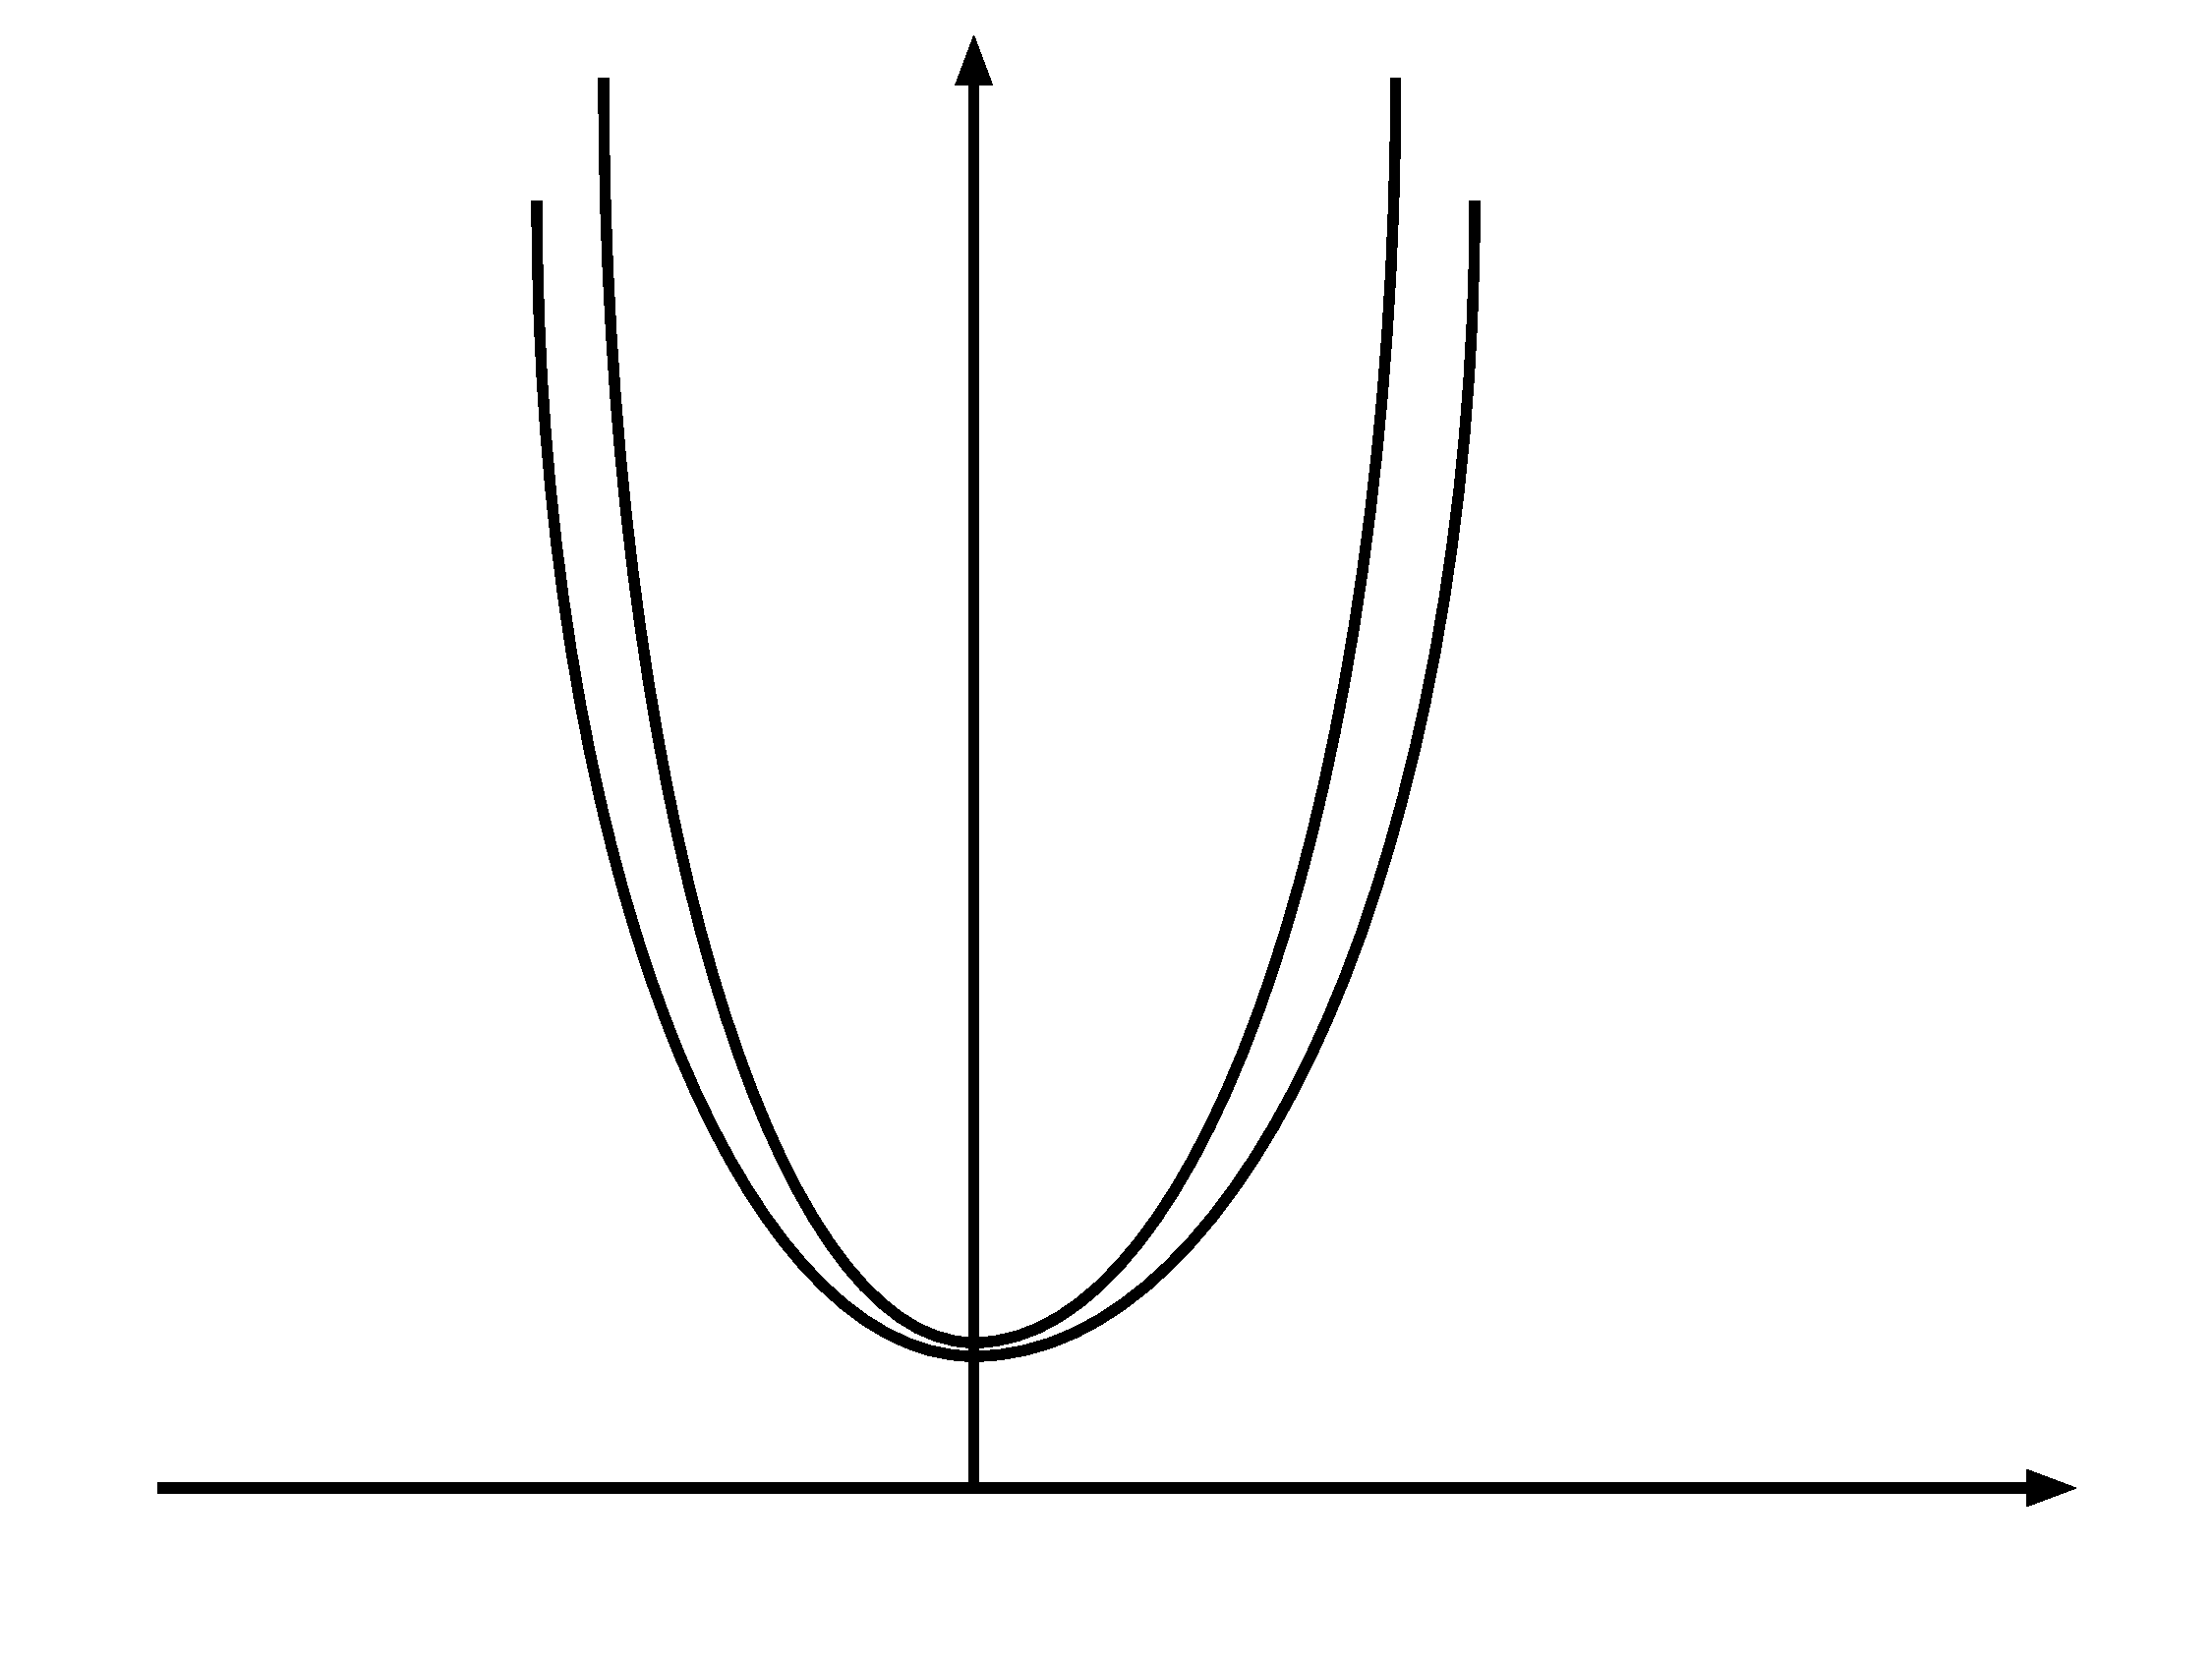
\includegraphics[width=0.6\textwidth,clip=true]{g0g1flow} 
\end{center}
\caption{Coupling constant $g$ as a function of $g$}
\label{fig:g0g1flow}
\end{figure}

\begin{figure}[t]
\begin{center}
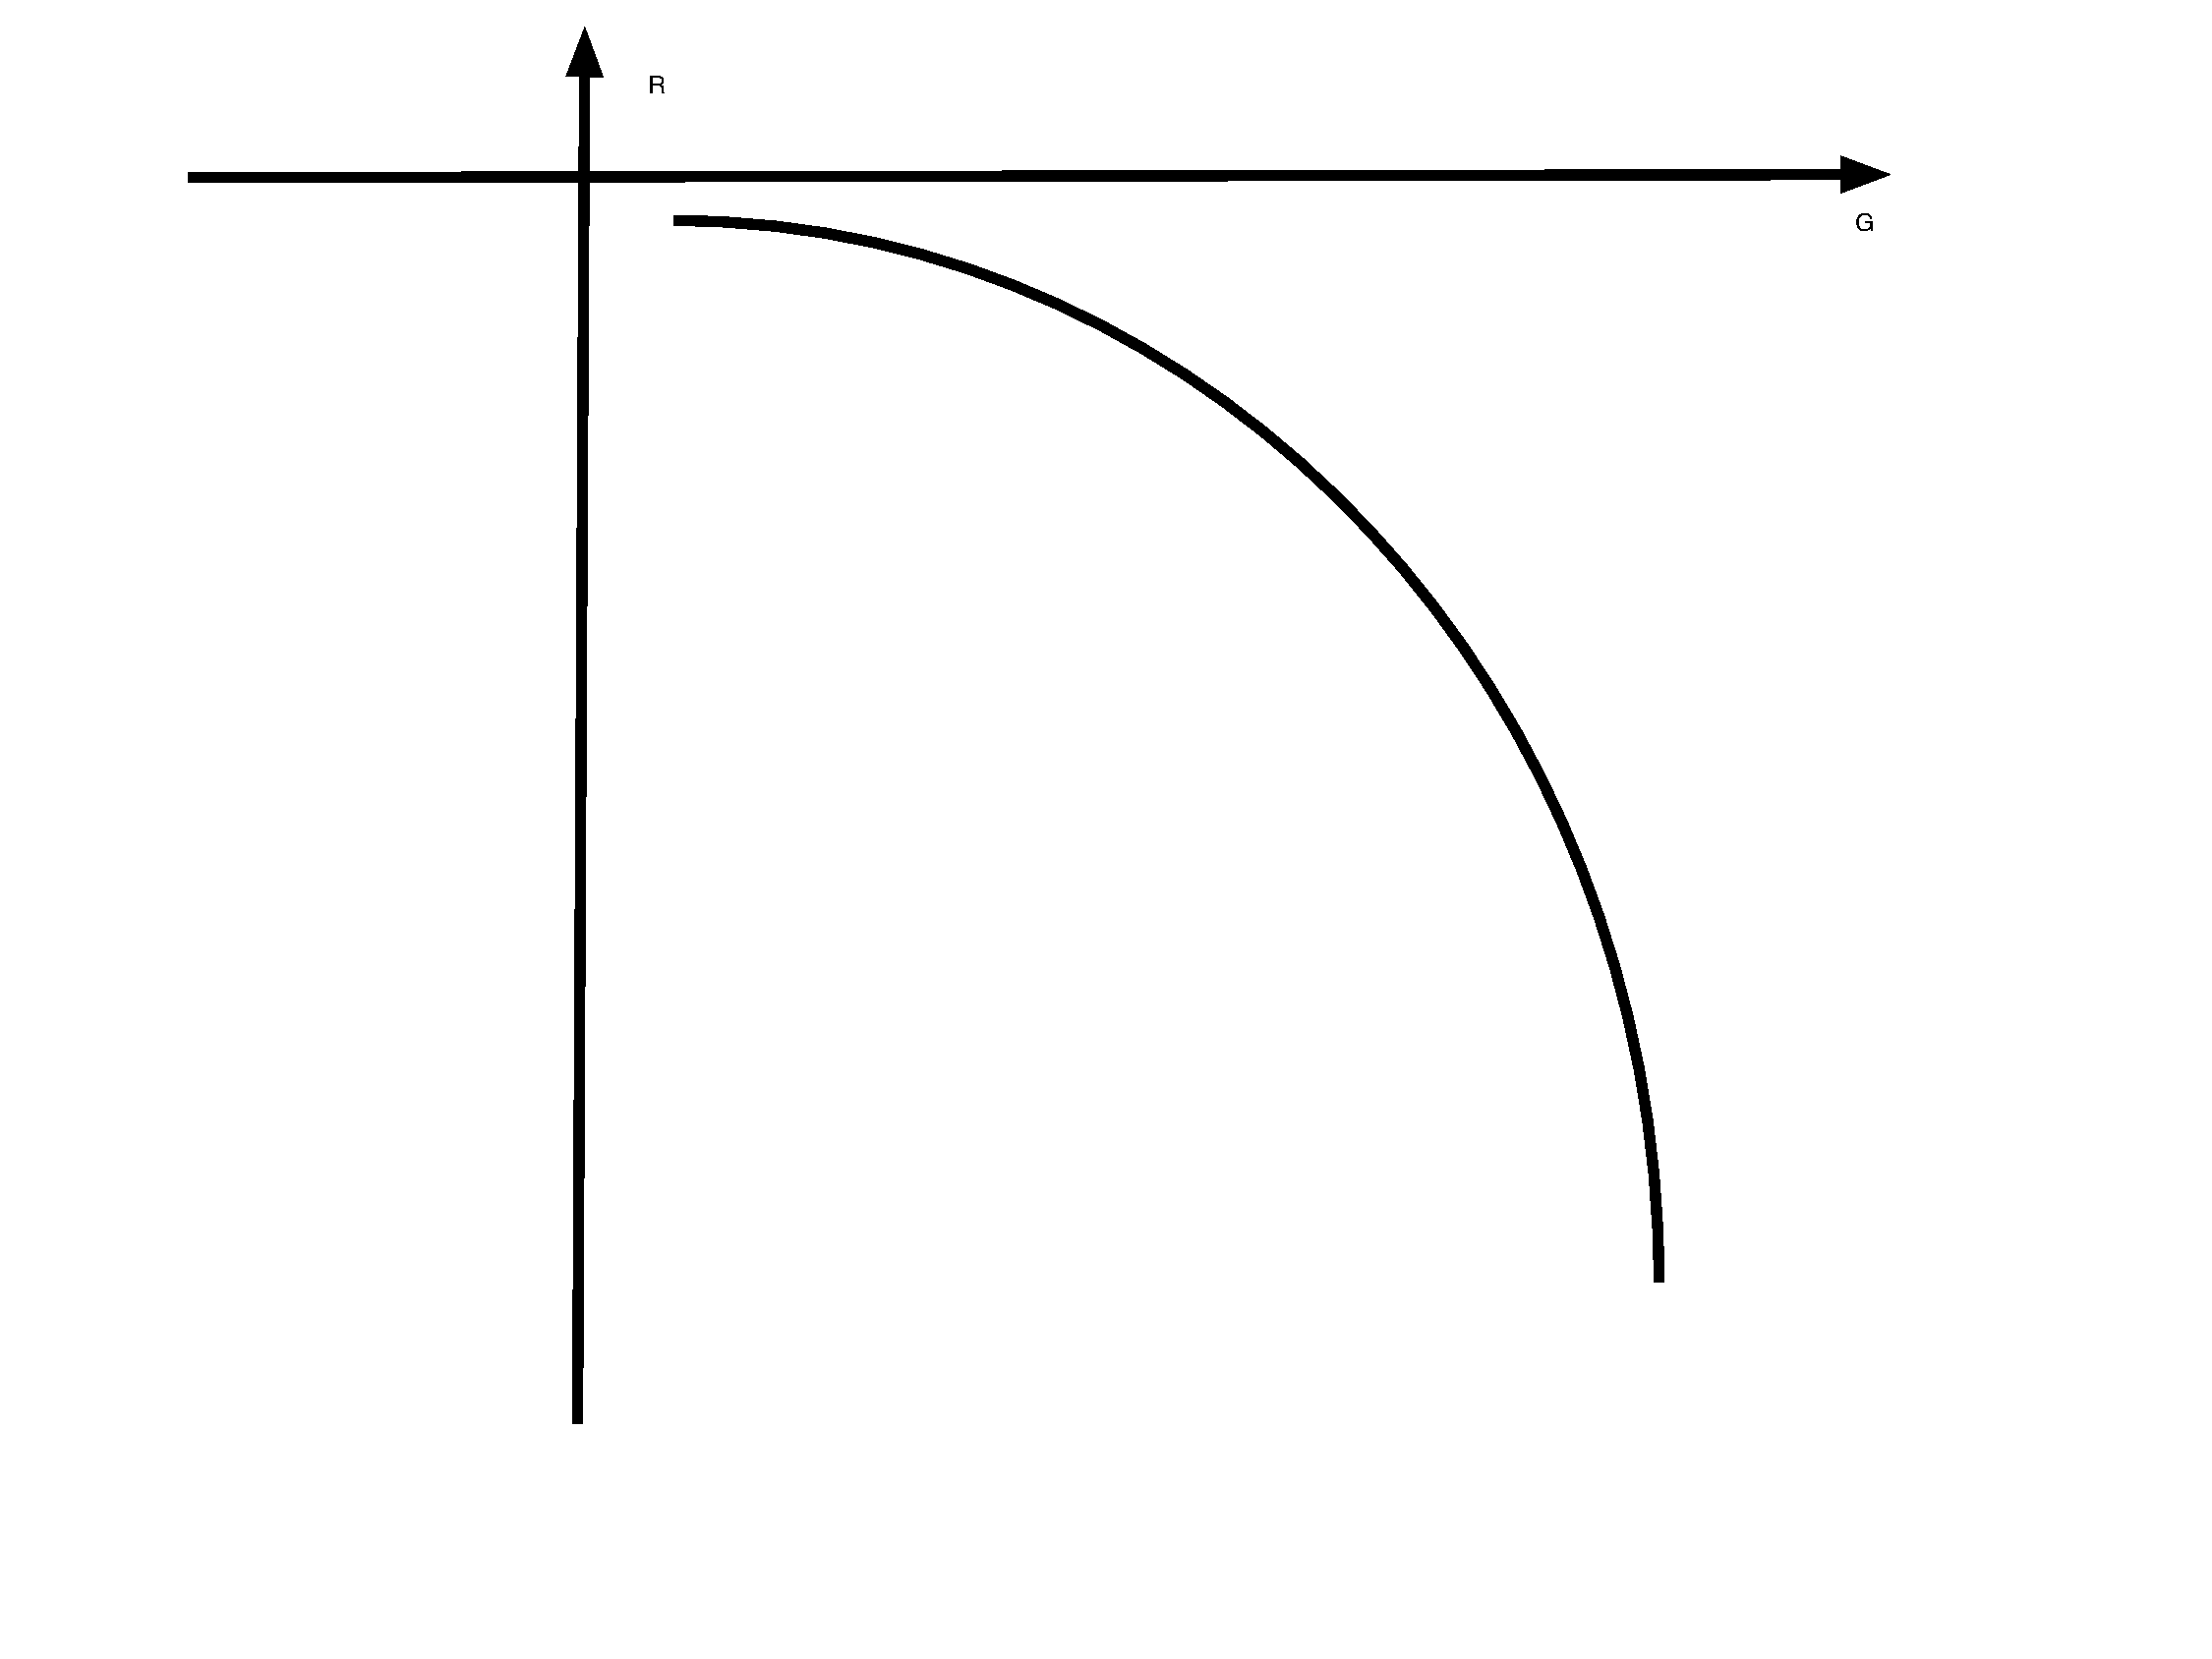
\includegraphics[width=0.6\textwidth,clip=true]{re-vs-g0} 
\end{center}
\caption{The $P$-wave effective range as a function of the coupling constant $g_0$}
\label{fig:Pwave-g0-re}
\end{figure}
\begin{acknowledgments}
  We thank H.-W. Hammer, D.~R.~Phillips, and S. K\"onig for useful discussions.
  This work has been supported by the National Science Foundation under Grant
  No. PHY-1555030, the Office of Nuclear Physics, U.S. Department of Energy
  under Contract No. DE-AC05-00OR22725, and the National Nuclear Security
  Administration No.~DE-NA0003883
\end{acknowledgments}


% * Bibiliography
\bibliographystyle{apsrev}
\bibliography{/Users/lplatter/Dropbox/References}
\end{document}

%%% Local Variables:
%%% mode: latex
%%% TeX-master: t
%%% End:
